\chapter{Aufgabe 3}

\noindent
Die in den Lösungsvorschlägen angegebene Reihenfolge dient nur zur Veranschaulichung und entspricht nicht notwendigerweise der in den Spezifikationen hinterlegten Reihenfolge.

\section{Teil a)}
IPSec im \textbf{Transportmodus} (s. Abbildung~\ref{fig:transportmodus}):

\begin{enumerate}
    \itemsep0.5em
    \item Der original IP-Header wird im \textbf{Transportmodus} beibehalten
    \item Erzeugung des IPSec-Headers, der je nach verwendetem IPSec-Protokoll aufgebaut ist (\textit{Authentication Header AH}~\cite{RFC4302} oder \textit{Encapsulating Security Payload ESP}~\cite{RFC4303}) - bei \textit{AH} und \textit{ESP} wird der \textit{HMAC} unter Berücksichtigung der Nutzdaten, des AH-Headers und Feldern des IP-Headers, die nicht geändert werden\footnote{
    bestimmte Felder eines IP-Headers unterliegen Änderungen, während sie von Knotenpunkt zu Knotenpunkt geleitet werden, wie bspw. das IPv4 \textit{TTL}-Feld (\textit{Time-To-Live},~\cite[360 ff.]{KR14}), und dürfen deshalb nicht zur Generierung des HMAC miteinbezogen werden.
    }, generiert

    \item Einbettung des IPSec-Headers nach dem originalen IP-Header
    \item Einbettung der Payloads nach dem IPSec-Header; im Fall von ESP: \textbf{verschlüsselt}
    \item Falls \textit{ESP} verwendet wird: Erzeugung und Anhängen des ESP-Trailers
\end{enumerate}


\begin{figure}
    \centering
    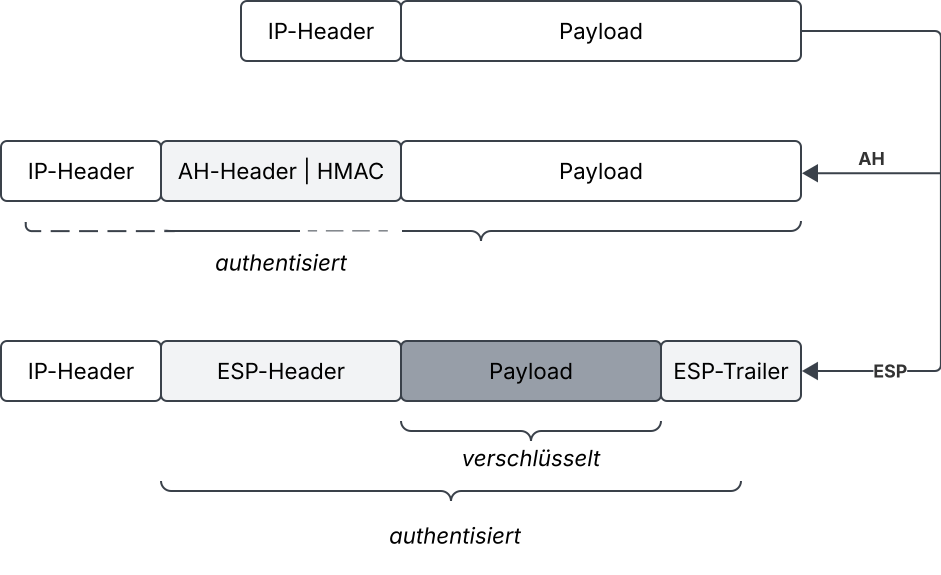
\includegraphics[scale=0.4]{aufgabe 3/img/transportmodus.svg}
    \caption{Skizze von IPSec im Transportmodus unter Anwendung von \textit{AH} bzw. \textit{ESP}. \textit{AH} sorgt für Authentizität und Integrität, während ESP durch die Verschlüsselung \textbf{zusätzlich} Vertraulichkeit garantiert. (Quelle: In Anlehnung an~\cite[\textbf{Abb. 3.6}, 41]{ITS4})}
    \label{fig:transportmodus}
\end{figure}

\noindent
Damit Vertraulichkeit garantiert ist, muss an dieser Stelle also \textbf{ESP} als Protokoll gewählt werden.
Damit \textbf{Spoofing} vermieden werden kann, sollte eine Kombination aus AH und ESP gewählt werden, da ansonsten der IP-Header nicht geschützt ist.

\section{Teil b)}
IPSec im \textbf{Tunnelmodus} (s. Abbildung~\ref{fig:tunnelmodus}):

\begin{enumerate}
    \itemsep0.5em
    \item Erzeugung eines neuen IP-Headers mit den Adressinformationen, insb. Zieladresse IPSec-Gateway
    \item Erzeugung des IPSec Headers (unter gleichen Bedingungen wie in Lösungsvorschlag zu Aufgabenteil a) angegeben)
    \item Einbettung des IPSec-Headers nach dem \textbf{neuen} IP-Header
    \item Kapselung des originalen IP-Headers und Payloads nach dem IPSec-Header (im Fall von ESP \textbf{verschlüsselt})
    \item Falls \textit{ESP} verwendet wird: Erzeugung und Anhängen des ESP-Trailers
\end{enumerate}

\begin{figure}
    \centering
    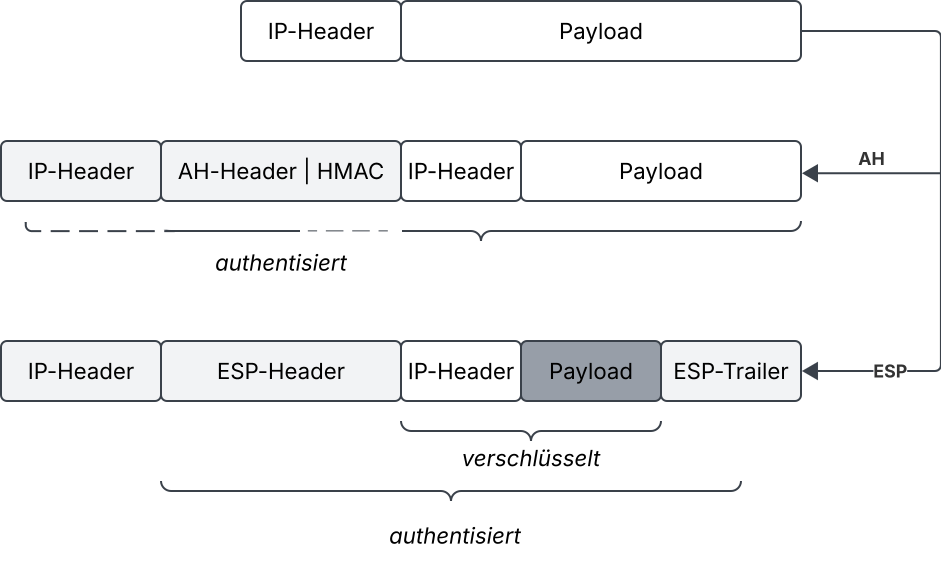
\includegraphics[scale=0.4]{aufgabe 3/img/tunnelmodus.svg}
    \caption{Skizze von IPSec im Tunnelmodus unter Anwendung von \textit{AH} bzw. \textit{ESP}. (Quelle: In Anlehnung an~\cite[\textbf{Abb. 3.6}, 41]{ITS4})}
    \label{fig:tunnelmodus}
\end{figure}

\noindent
Auch hier gilt: Damit Vertraulichkeit garantiert ist, muss an dieser Stelle \textbf{ESP} als Protokoll gewählt werden.
Da der Tunnelmodus verwendet wird, ist eine zusätzliche Absicherung durch AH wie im Transportmodus in dem geg.
Kontext nicht notwendig: Das ursprüngliche IP-Paket (inkl. Header) wird gekapselt und verschlüsselt, Manipulationen daran sind über die Authentisierungsmechanismen von ESP erkennbar.

\section{Teil c)}

\textit{Wenn auf beiden Seiten ein IPSec‐Gateway die bidirektionale Weiterleitung der
Datenströme erledigen soll, wie viele Sicherheitsassoziationen sind dann für die
jeweiligen Lösungen zu a) und b) notwendig?}\\

\noindent
Die SAs (\textit{Security Associations}) sind \textit{unidirektional}: Es können also SAs für hereinkommende und herausgehende Pakete festgelegt werden (vgl.~\cite[773]{Eck18}).\\

\noindent
Es werden u.a. folgende Informationen von den SAs verwaltet, was sowohl für den Tunnelmodus als auch den Transportmodus  gilt:

\begin{itemize}
    \item \textbf{AH-Protokoll}: Signaturverfahren
    \item \textbf{ESP-Protokoll}: Verschlüsselungsverfahren, Schlüssel
\end{itemize}

\noindent
Somit sind jeweils mindestens eine SA für AH und mindestens eine SA für ESP notwendig.
Werden die Verfahren kombiniert, ergibt sich in Summe also zwei SAs.\\

\noindent
\textbf{Beispiel}:
Empfänger $A$ nutzt zum Versenden an $B$ die Protokolle AH und ESP in Kombination.\\
Damit $B$ die Informationen verarbeiten kann, benötigt $B$ \textbf{zwei} SAs.\\
Versendet $B$ hingegen nur unter Verwendung von AH, benötigt $A$ nur eine SA.
Für diese Art der bidirektionalen Kommunikation werden also 3 SAs benötigt.

\noindent
Entsprechend berechnet sich die Anzahl aus den eingesetzten Verfahren für jede Kommunikationsrichtung: Verwenden $A$ und $B$ jeweils nur AH sind insgesamt nur zwei SAs notwendig, verwenden $A$ und $B$ jeweils AH und ESP sind insgesamt 4 notwendig usw.\footnote{
    Anzumerken ist an dieser Stelle, dass IPSec i.A. nicht symmetrisch sein muss: So kann sich eine Seite auch dazu entscheiden, unter Anwendung von IPSec nur zu empfangen, aber nicht notwendigerweise auch zu versenden.
}\\

\noindent
Da in dem Aufgabenteil a) die  Verwendung von ESP und AH zur Sicherstellung von Vertraulichkeit und Integrität empfohlen wurde, erhalten wir in Summe $4$ SAs.
Da in dem Aufgabenteil b) die verwendung von ESP empfohlen wurde, erhalten wir in Summe $2$ SAs.\\


\section{Teil d)}

\textit{Welche Sicherheitseigenschaften bietet die Lösung b) zusätzlich zu den geforderten.}

\noindent
Durch die Verwendung des Tunnelmodus ist insgesamt der tatsächliche Endpunkt der Kommunikation zwischen $A$ und $B$ für einen Angreifer transparent - er könnte allerhöchstens die Endpunkte der IPSec-Gateways ermitteln.\\
Dadurch lässt sich effizient eine \textbf{Verkehrsflussanalyse} verhindern (vgl.~\cite[46]{ITS4}).